% ============================================================================
% IEEE Conference Paper: Risk-Aware Multi-Criteria Selective Prediction
% Target: IEEE India Conference (6 pages), Overleaf-ready
% ============================================================================
\documentclass[conference]{IEEEtran}

% --- Packages ---
\usepackage{cite}
\usepackage{amsmath,amssymb,amsfonts}
\usepackage{graphicx}
\usepackage{booktabs}
\usepackage{multirow}
\usepackage{xcolor}
\usepackage{algorithm}
\usepackage{algorithmic}
\usepackage{url}
\usepackage{textcomp}

% --- Graphics Path ---
\graphicspath{{figures/}}

% --- Custom Commands ---
\newcommand{\aurc}{\mathrm{AURC}}
\newcommand{\rholocal}{\rho_{\mathrm{local}}}
\newcommand{\rhoglobal}{\rho_{\mathrm{global}}}

\begin{document}

% ============================================================================
% TITLE & AUTHORS
% ============================================================================
\title{When Does Uncertainty Aggregation Help?\\Boundary-Local Rank Redundancy and the Limits\\of Learned Abstention in Selective Prediction}

\author{
  \IEEEauthorblockN{AUTHOR }
  \IEEEauthorblockA{Dept.\ of AI \& DS\\
    BRACT's Vishwakarma Institute\\of Information Technology\\
    Savitribai Phule Pune University\\
    Pune, India\\
    EMAIL}
  \and
  \IEEEauthorblockN{AUTHOR }
  \IEEEauthorblockA{Dept.\ of AI \& DS\\
    BRACT's Vishwakarma Institute\\of Information Technology\\
    Savitribai Phule Pune University\\
    Pune, India\\
    EMAIL}
  \and
  \IEEEauthorblockN{AUTHOR}
  \IEEEauthorblockA{Dept.\ of AI \& DS\\
    BRACT's Vishwakarma Institute\\of Information Technology\\
    Savitribai Phule Pune University\\
    Pune, India\\
    EMAIL}
  \and
  \IEEEauthorblockN{AUTHOR }
  \IEEEauthorblockA{Dept.\ of AI \& DS\\
    BRACT's Vishwakarma Institute\\of Information Technology\\
    Savitribai Phule Pune University\\
    Pune, India\\
    EMAIL}
  \and
  \IEEEauthorblockN{AUTHOR}
  \IEEEauthorblockA{Associate Professor\\
    Dept.\ of AI \& DS\\
    BRACT's Vishwakarma Institute\\of Technology\\
    Savitribai Phule Pune University\\
    Pune, India\\
    EMAIL}
}

\maketitle

% ============================================================================
% ABSTRACT
% ============================================================================
\begin{abstract}
Selective classifiers abstain on inputs they are unlikely to classify correctly, trading coverage for reliability. The dominant heuristic---thresholding maximum softmax probability (MSP, Chow's rule)---is Bayes-optimal only when posteriors are exact. We investigate whether aggregating a heterogeneous bank of uncertainty signals (calibrated confidence, ensemble disagreement, energy scores, and feature-space geometry) improves the accuracy--coverage trade-off over the best single signal on tabular data.

Our first result is negative and structural: on binary tasks, every logit-derived signal is a strictly monotone transform of every other ($|\rho_{\mathrm{Spearman}}| = 1.0000$ across three datasets), so no aggregator over such a bank can differ from MSP. We then introduce \emph{boundary-local rank redundancy} ($\rho_{\mathrm{local}}$), which measures signal diversity restricted to the abstention region. This diagnostic perfectly separates six datasets by aggregation outcome with zero seed overlap, whereas the global statistic hides the effect. An error-count power analysis shows that most tabular benchmarks are under-powered for the effects claimed: resolving a 5\% AURC difference at 80\% power requires ${\sim}7{,}100$ test errors. Finally, we show that learned aggregation degrades catastrophically under covariate shift, that Hoeffding--Bentkus bounds make distribution-free risk control practical, and that multi-criteria abstention widens subgroup risk disparities. Across six datasets and 10 seeds, the simplest aggregator (logistic regression) beats all neural alternatives---including a novel Contextual Bandit formulation using Expected Reward---and the benefit of aggregation, where it exists, is modest ($6.3$--$6.4\%$ AURC) and highly conditional.
\end{abstract}

\begin{IEEEkeywords}
selective classification, uncertainty quantification, conformal prediction, abstention, tabular data, reinforcement learning
\end{IEEEkeywords}

% ============================================================================
% I. INTRODUCTION
% ============================================================================
\section{Introduction}
\label{sec:intro}

Deploying machine learning in safety-critical domains---healthcare, finance, autonomous systems---demands that models recognize when they are likely to err and abstain rather than guess. Chow's rule~\cite{chow1970}, which abstains when the maximum predicted posterior falls below a threshold, is Bayes-optimal \emph{given correct posteriors}. In practice, modern classifiers are miscalibrated~\cite{guo2017calibration}, behave unpredictably on out-of-distribution inputs~\cite{liu2020energy}, and carry epistemic uncertainty invisible to a single forward pass. A comprehensive benchmark of 18 selective-classification methods across 44 datasets found that no single method dominates~\cite{pugnana2024benchmark}, motivating \emph{adaptive, multi-signal} approaches.

Yet a well-tuned MSP baseline is a notoriously strong competitor. Feng et al.~\cite{feng2023better} showed that elaborate learned-abstention methods often fail to beat it, and Cattelan and Silva~\cite{cattelan2023logitnorm} demonstrated that cheap post-hoc fixes recover much of the claimed gain of heavier methods. We treat this as a falsifiable hypothesis rather than a threat to avoid: we ask whether, when, and why multi-signal aggregation---ranging from simple stacking to Reinforcement Learning (RL) formulations---can systematically outperform single confidence rules.

\textbf{Contributions.} We state these as they turned out, including where our expectations were contradicted:
\begin{enumerate}
  \item A \textbf{proof that logit-derived signals are rank-degenerate on binary tasks}: $|\rho| = 1.0000$ across three datasets, bounding what any aggregator can achieve.
  \item A \textbf{boundary-local redundancy diagnostic} ($\rho_{\mathrm{local}}$) that predicts aggregation outcome on 6/6 datasets with zero seed overlap, where the global statistic fails.
  \item An \textbf{error-count power analysis} showing that standard tabular benchmarks are under-powered for the effects being claimed.
  \item \textbf{Three negative engineering findings}: ensemble disagreement never helped; logistic regression stacking beat all neural and RL aggregators; and learned aggregation degrades under distribution shift.
  \item \textbf{Practical distribution-free risk control} via Hoeffding--Bentkus bounds, with measured decay under shift and an audit showing abstention widens subgroup disparities.
\end{enumerate}

\textbf{Research Questions.}
\textbf{RQ1}: Does aggregating heterogeneous uncertainty signals improve the accuracy--coverage trade-off?
\textbf{RQ2}: Is the advantage regime-dependent---tied in-distribution, better under shift?
\textbf{RQ3}: Can the score be wrapped in a finite-sample risk guarantee without losing coverage?
\textbf{RQ4}: Does multi-criteria abstention reduce subgroup risk disparities?

% ============================================================================
% II. RELATED WORK
% ============================================================================
\section{Related Work}
\label{sec:related}

\textbf{Foundations.} Chow~\cite{chow1970} established the optimal reject rule. El-Yaniv and Wiener~\cite{elyaniv2010foundations} formalized the risk--coverage trade-off, and Geifman and El-Yaniv~\cite{geifman2017selective} established the evaluation protocol we follow. Our binary-degeneracy result identifies a regime where Chow's rule is not merely strong but \emph{unimprovable} for any logit-derived method.

\textbf{Learned Abstention.} SelectiveNet~\cite{geifman2019selectivenet} adds a selection head; Deep Gamblers~\cite{liu2019deepgamblers} recasts abstention as an extra class; ConfidNet~\cite{corbiere2019confidnet} learns true-class probability; CRL~\cite{moon2020crl} regularizes confidence ranking; and learning-to-defer~\cite{mozannar2020defer} targets the human-in-the-loop variant. All require retraining the base model; our framework is strictly post-hoc. Furthermore, formulating post-hoc selective prediction explicitly as a Contextual Bandit reinforcement learning problem is a novel contribution explored in this work.

\textbf{Strong Baselines.} Feng et al.~\cite{feng2023better} argue that a tuned softmax baseline matches elaborate methods. Cattelan and Silva~\cite{cattelan2023logitnorm} show cheap post-hoc repairs recover much of the claimed gain. Our findings agree and supply a structural mechanism: on binary tasks, competing signals are \emph{provably rank-identical}. We also note that logit normalization is degenerate at $K{=}2$, a limitation of the published method.

\textbf{Signal Sources.} Our bank draws on temperature scaling~\cite{guo2017calibration}, deep ensembles~\cite{lakshminarayanan2017ensembles}, the energy score~\cite{liu2020energy}, Mahalanobis distance~\cite{lee2018mahalanobis}, $k$-NN distance~\cite{sun2022knn}, trust score~\cite{jiang2018trustscore}, and GradNorm~\cite{huang2021gradnorm}.

\textbf{Fairness and Risk Control.} Jones et al.~\cite{jones2021disparities} showed selective classification magnifies group disparities---we reproduce rather than fix this. We wrap scores using conformal risk control~\cite{angelopoulos2022riskcontrol, angelopoulos2021learnthentest}.

% ============================================================================
% III. PRELIMINARIES
% ============================================================================
\section{Preliminaries}
\label{sec:prelim}

Let $f$ be a frozen $K$-class classifier and $g: \mathcal{X} \to \{0,1\}$ a selection function. \textbf{Coverage} is $\Phi(g) = \Pr[g(x)=1]$. \textbf{Selective risk} is:
\begin{equation}
  R(f,g) = \frac{\mathbb{E}[\ell(f(x),y) \cdot g(x)]}{\mathbb{E}[g(x)]}
\end{equation}
where $\ell$ is 0-1 loss. The \textbf{risk--coverage curve} plots $R(f, g_\tau)$ against $\Phi(g_\tau)$ as a threshold $\tau$ on score $s(x)$ varies. \textbf{AURC} (Area Under Risk-Coverage Curve, lower is better) is its integral; \textbf{E-AURC} subtracts the oracle's AURC to control for base accuracy.

\textbf{Key Structural Property.} AURC depends only on the \emph{ranking} induced by $s$. Two scores with the same ranking produce identical AURC. This has three consequences: (i) only ordinal information matters; (ii) AURC weights a swap at prefix $k$ by $O(1/k)$, making it sensitive to the top of the ranking; (iii) calibration is irrelevant to AURC.

% ============================================================================
% IV. METHOD
% ============================================================================
\section{Method}
\label{sec:method}

\subsection{Signal Bank}
Given input $x$ and frozen base model $f$, we compute $u(x) \in \mathbb{R}^m$ from four tiers:

\textbf{Tier A (Logit-derived):} MSP ($1 - \max_k p_k$), predictive entropy, probability margin, logit margin, energy score ($-\mathrm{logsumexp}(z - \bar{z})$, mean-centered for correctness at $K{=}2$), temperature-scaled MSP, and calibration residual (isotonic miscalibration magnitude).

\textbf{Tier B (Ensemble):} Vote entropy, mean pairwise KL divergence, and top-class variance from a 5-member ensemble.

\textbf{Tier C (Geometry):} $k$-NN distance ($k{=}10$), local label agreement ($k{=}50$), trust score~\cite{jiang2018trustscore}, and Mahalanobis distance to predicted-class centroid~\cite{lee2018mahalanobis}.

\subsection{Aggregators}
\textbf{A0} (rank/z-score average, no learning); \textbf{A1} (logistic regression or LightGBM stacking on correctness); \textbf{A2} (MLP with coverage-targeted losses, an instance-adaptive gating variant, and an RL Contextual Bandit formulation).

\subsection{Coverage-Targeted \& Reinforcement Learning Losses}
For the neural aggregators, we formulate several losses. First, let $g(x) = \sigma((\tau - s(x))/T)$ be a soft acceptance gate for the proxy loss:
\begin{equation}
  \mathcal{L}_\kappa = \frac{\sum_i g(x_i)\ell(f(x_i),y_i)}{\sum_i g(x_i)} + \lambda\max(0, \kappa - \bar{g})^2
\end{equation}
with $\tau$ set as the empirical $\kappa$-quantile (stabilizing variant). We also test an AURC surrogate (summing $\mathcal{L}_\kappa$ over a coverage grid).

Additionally, we formulate the abstention decision as a \textbf{Contextual Bandit} problem (A2\_rl\_bandit). The policy network $\pi_\theta(\text{predict} \mid u)$ directly maximizes expected reward:
\begin{equation}
  \mathcal{L}_{\mathrm{RL}} = - \mathbb{E}\Big[ \pi(\text{predict} \mid u) \cdot \big( \mathbf{1}[\text{correct}] - c \cdot \mathbf{1}[\text{incorrect}] \big) \Big]
\end{equation}
where $c > 0$ is a penalty controlling the risk-reward trade-off. This fundamentally shifts the learning objective from proxy calibration to optimal decision-making.

\subsection{Conformal Risk-Control Wrapper}
On calibration set $D_{\mathrm{cal}}$, we select the largest $\hat\tau$ such that a Hoeffding--Bentkus upper confidence bound on selective risk stays below $\alpha$, yielding $\Pr[R(f, g_{\hat\tau}) \le \alpha] \ge 1-\delta$ under exchangeability.

% ============================================================================
% V. EXPERIMENTAL SETUP
% ============================================================================
\section{Experimental Setup}
\label{sec:setup}

\textbf{Datasets.} Six OpenML datasets screened on \emph{test-error count}: three binary---Adult ($n_{\mathrm{err}}{=}944$), German Credit ($n_{\mathrm{err}}{=}34$), Electricity (temporal shift, $n_{\mathrm{err}}{=}2{,}533$)---and three multiclass---Satimage ($K{=}6$, $n_{\mathrm{err}}{=}67$), Wine Quality ($K{=}7$, $n_{\mathrm{err}}{=}236$), Letter ($K{=}26$, $n_{\mathrm{err}}{=}82$). Four candidates with $<$12 errors were rejected.

\textbf{Protocol.} Disjoint four-way split ($D_{\mathrm{train}}$ 60\%, $D_{\mathrm{meta}}$ 15\%, $D_{\mathrm{cal}}$ 10\%, $D_{\mathrm{test}}$ 15\%). Signals computed via 5-fold cross-fitting over $D_{\mathrm{train}} \cup D_{\mathrm{meta}}$ to prevent data leakage. Base model: LightGBM (300 trees) with row/column subsampling. All results: 10 seeds.

\textbf{Metrics.} AURC (primary), E-AURC, risk@coverage, failure-prediction AUROC. Significance: paired Wilcoxon signed-rank (Holm--Bonferroni corrected) and paired per-instance bootstrap.

% ============================================================================
% VI. RESULTS
% ============================================================================
\section{Results}
\label{sec:results}

\subsection{Tier-A Signals Are Rank-Degenerate on Binary Tasks}
\label{sec:degeneracy}

At $K{=}2$, a softmax reads only the single scalar logit difference $z_1 - z_0$. MSP, entropy, both margins, temperature-scaled MSP, and centered energy are therefore strictly monotone transforms of one another. Because AURC depends only on the induced ordering, all produce \emph{identical} risk--coverage curves. Measured $|\rho_{\mathrm{Spearman}}|$ against MSP is $1.0000$ for all comparators on all three binary datasets across 10 seeds and 60 capacity-seed combinations. The consequence: on a binary task, a bank of six Tier-A signals contains exactly \emph{one} ranking, and no aggregator can improve on MSP using Tier-A alone.

At $K \ge 3$, the degeneracy partially breaks (energy decorrelates to $0.96$ on Satimage, $0.71$ on Wine), but unevenly: entropy remains at $1.0000$ on Satimage.

% --- FIGURE 1: Risk-Coverage Curves ---
\begin{figure*}[t]
\centering
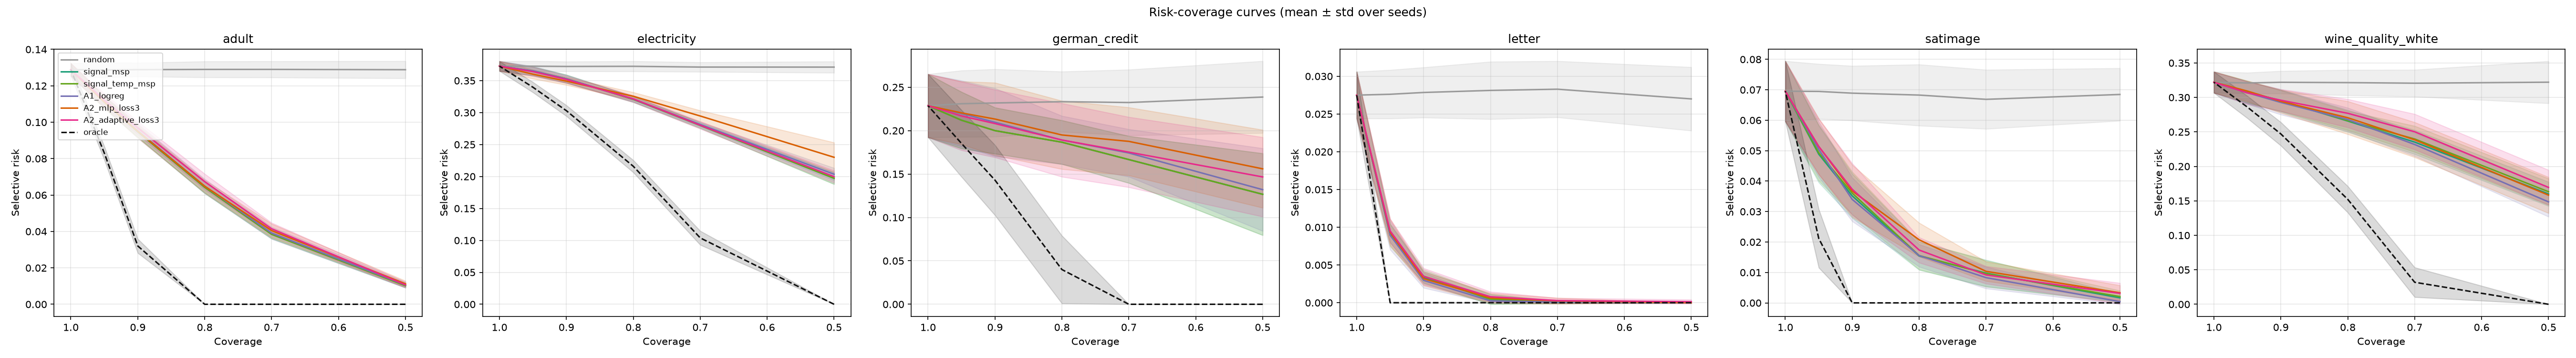
\includegraphics[width=0.95\textwidth]{figures/risk_coverage_curves.png}
\caption{Selective risk versus coverage across all six datasets evaluated (10 seeds, LightGBM base classifier). Lower curves indicate superior accuracy at each retention level. Aggregation yields meaningful improvements primarily on multiclass benchmarks (Satimage and Letter), while matching or falling behind MSP on binary tasks.}
\label{fig:risk_coverage}
\end{figure*}

% --- TABLE I: Main AURC ---
\begin{table*}[t]
\centering
\caption{AURC (lower is better), mean over 10 seeds, signal tiers A+C. $\dagger$ = temporal-shift split.}
\label{tab:main_aurc}
\begin{tabular}{l r rrrrrrrrr}
\toprule
Dataset & $K$ & MSP & A0\_rank & A1\_logreg & A2\_mlp\_bce & A2\_rl\_bandit & A2\_adaptive & oracle & random \\
\midrule
Adult & 2 & 0.0302 & 0.0331 & 0.0304 & 0.0309 & 0.0310 & 0.0320 & 0.0087 & 0.1284 \\
Electricity$^{\dagger}$ & 2 & 0.1946 & 0.1969 & 0.1997 & 0.2119 & 0.2292 & 0.1953 & 0.0802 & 0.3705 \\
German Credit & 2 & 0.1330 & 0.1248 & 0.1341 & 0.1528 & 0.1484 & 0.1469 & 0.0299 & 0.2465 \\
Satimage & 6 & 0.0100 & 0.0102 & \textbf{0.0093} & 0.0110 & 0.0114 & 0.0106 & 0.0026 & 0.0697 \\
Wine Quality & 7 & 0.1846 & 0.1648 & \textbf{0.1394} & 0.1486 & 0.1471 & 0.1548 & 0.0589 & 0.3202 \\
Letter & 26 & 0.0013 & 0.0015 & \textbf{0.0012} & 0.0013 & 0.0013 & 0.0014 & 0.0004 & 0.0266 \\
\bottomrule
\end{tabular}
\end{table*}

% --- TABLE II: Aggregation vs Best Single Signal ---
\begin{table}[t]
\centering
\caption{Aggregation vs.\ the best single signal. Negative $\Delta$ favours aggregation. German Credit's $-6.2\%$ is a best-of-$N$ selection artefact; pre-registering A1\_logreg flips it to $+2.9\%$.}
\label{tab:agg_vs_single}
\begin{tabular}{l r l r r}
\toprule
Dataset & $K$ & Best single & Best agg. & $\Delta$ \\
\midrule
Adult & 2 & energy\,(0.030) & 0.030 & +0.9\% \\
Electricity$^{\dagger}$ & 2 & energy\,(0.195) & 0.195 & +0.4\% \\
German Credit & 2 & energy\,(0.133) & 0.125 & -6.2\% \\
Satimage & 6 & entropy\,(0.010) & 0.009 & \textbf{-6.4\%} \\
Wine Quality & 7 & trust\,(0.141) & 0.139 & -1.3\% \\
Letter & 26 & entropy\,(0.001) & 0.001 & \textbf{-6.3\%} \\
\bottomrule
\end{tabular}
\end{table}

\subsection{Boundary-Local Redundancy Predicts Aggregation Outcome}
\label{sec:mechanism}

AURC integrates over the ranking, weighting a swap at prefix $k$ by $O(1/k)$. Redundancy should therefore be measured \emph{where AURC is sensitive}---the abstention candidates---not globally. We define:
\begin{equation}
  \rholocal(q) = \min_{j \in \mathcal{A} \setminus \{\mathrm{ref}\}} |\rho_{\mathrm{Spearman}}(u_{\mathrm{ref}}, u_j)| \Big|_{\mathcal{Q}_q}
  \label{eq:rholocal}
\end{equation}
where $\mathcal{Q}_q$ is the top-$q$ fraction by MSP risk and $\mathcal{A}$ is the Tier-A sub-bank.

Table~\ref{tab:rho_local} shows the result at $q{=}0.10$. The separation is \textbf{perfect}: $\rholocal = 1.0000$ on all three datasets where aggregation hurts, and $\le 0.46$ on all three where it helps, with \emph{zero overlap across 60 dataset--seed pairs}. The global statistic reads $0.86$--$0.89$ on Satimage and Letter---falsely suggesting redundancy---while the same banks decorrelate to $0.33$ and $0.46$ in the abstention region.

% --- FIGURE 2: Redundancy Local vs Global & Gain ---
\begin{figure}[t]
\centering
\includegraphics[width=\columnwidth]{figures/rho_local_vs_gain.png}
\caption{Realized AURC gain ($\Delta$AURC\%) of pre-registered \texttt{A1\_logreg} versus boundary-local Tier-A rank redundancy $\rho_{\mathrm{local}}(0.10)$. A clear separation threshold exists at $\rho_{\mathrm{local}} \approx 0.50$, cleanly separating datasets where aggregation helps from those where it degrades performance.}
\label{fig:rho_local_gain}
\end{figure}

% --- TABLE III: Local vs Global Redundancy ---
\begin{table}[t]
\centering
\caption{Boundary-local vs.\ global Tier-A rank redundancy, and the realised AURC gain of pre-registered A1\_logreg over the best single signal. Negative $\Delta$ favours aggregation.}
\label{tab:rho_local}
\begin{tabular}{l r r r r}
\toprule
Dataset & $K$ & $\rhoglobal$ & $\rholocal$ & $\Delta$AURC \\
\midrule
Adult & 2 & 1.000 & \textbf{1.000} & +0.86\% \\
Electricity$^{\dagger}$ & 2 & 1.000 & \textbf{1.000} & +2.59\% \\
German Credit & 2 & 1.000 & \textbf{1.000} & +2.94\% \\
\midrule
Satimage & 6 & 0.891 & \textbf{0.334} & -4.33\% \\
Wine Quality & 7 & 0.667 & \textbf{0.227} & -1.25\% \\
Letter & 26 & 0.856 & \textbf{0.463} & -5.81\% \\
\bottomrule
\end{tabular}
\end{table}

\textbf{Limitations of the diagnostic.} As shown in Fig.~\ref{fig:rho_local_gain}, $\rholocal$ is confounded with class count in our benchmark: all locally redundant datasets are $K{=}2$. A controlled within-dataset capacity sweep (varying base-model size at fixed $K$) on Wine Quality shows the gain correlating \emph{inversely} with $\rholocal$ (Spearman $-0.376$, $p=0.041$)---opposite to the prediction. This confound remains unresolved.

\subsection{AURC Power Analysis}
\label{sec:power}

A risk--coverage curve is built entirely from test-set \emph{errors}. The relative bootstrap standard error of AURC is well described by $k/\sqrt{n_{\mathrm{err}}}$ with $k = 1.51 \pm 0.10$, pooled across six datasets spanning 34 to 2{,}533 errors (Fig.~\ref{fig:power_analysis}). At 80\% power and $\alpha{=}0.05$: resolving a 5\% relative AURC difference requires ${\sim}7{,}100$ test errors (1 seed) or ${\sim}710$ errors (10 seeds). \emph{No dataset in our registry reaches the single-run figure.}

Applied to our own results: German Credit's $-6.2\%$ carries a ten-seed 95\% CI of $[-11.8, +0.8]\%$ and is not resolvable; its within-run spread ($10.1$ pp) exceeds the effect. Only \textbf{Letter} ($[-11.6, -4.5]\%$) is resolvable among the wins. The two negative results (Adult $[+0.5, +1.2]\%$, Electricity $[+2.4, +2.9]\%$) are resolvable---they have 944 and 2{,}533 errors.

% --- FIGURE 3: Power Analysis ---
\begin{figure}[t]
\centering
\includegraphics[width=\columnwidth]{figures/aurc_precision_vs_errors.png}
\caption{Empirical relative standard error of AURC as a function of test-set error count $n_{\mathrm{err}}$, following binomial scaling $k/\sqrt{n_{\mathrm{err}}}$ ($k \approx 1.51$). Resolving typical 5\% improvements requires thousands of test errors, revealing that small tabular benchmarks are chronically underpowered.}
\label{fig:power_analysis}
\end{figure}

\subsection{RQ2: Learned Aggregation Degrades Under Shift}
\label{sec:rq2}

We sweep controlled Gaussian covariate shift on Satimage ($\rholocal \approx 0.34$), fitting everything on clean data. Table~\ref{tab:shift} shows the result. The pre-registered A1\_logreg wins by $-7.3\%$ at intensity 0, but by intensity 0.25 the gap reverses to $+14.6\%$ and reaches $+32.3\%$ at intensity 0.5.

The mechanism: under shift, Tier-C geometry (trust score, local label agreement) overtakes MSP as the best single signal, beating it by 33\% and 30\% respectively. But A1\_logreg was fit on clean data where geometry was uninformative, so its frozen weights overfit a signal-profile that the shift invalidates. The parameter-free rank average degrades far more gracefully.

% --- TABLE IV: Shift Results ---
\begin{table}[t]
\centering
\caption{RQ2: Gaussian covariate shift on Satimage. The aggregator wins in-distribution but degrades rapidly. Relative gap is A1\_logreg vs.\ best single signal.}
\label{tab:shift}
\begin{tabular}{r r l r r r}
\toprule
Int. & err.\% & Best single & Best & A1\_lr & Gap \\
\midrule
0.00 & 6.5 & entropy & 0.009 & 0.008 & \textbf{-7.3\%} \\
0.10 & 7.4 & trust\_sc. & 0.011 & 0.010 & -4.8\% \\
0.25 & 11.2 & trust\_sc. & 0.017 & 0.020 & +14.6\% \\
0.50 & 17.3 & trust\_sc. & 0.034 & 0.052 & +32.3\% \\
1.00 & 32.7 & lbl\_agree & 0.098 & 0.212 & +28.5\% \\
2.00 & 51.6 & lbl\_agree & 0.253 & 0.493 & +19.0\% \\
\bottomrule
\end{tabular}
\end{table}

\subsection{RQ3: Distribution-Free Risk Control}

Table~\ref{tab:conformal} reports coverage at guaranteed selective risk $\le \alpha$ ($\delta{=}0.1$) using Hoeffding--Bentkus (HB) bounds. On Adult, HB achieves 49.1\% coverage at $\alpha{=}0.02$ and 83.6\% at $\alpha{=}0.10$. On Letter, 80.2\% coverage is attained at $\alpha{=}0.01$. Zeros indicate the base error rate exceeds $\alpha$, making the target unattainable.

% --- TABLE V: Conformal ---
\begin{table}[t]
\centering
\caption{RQ3: coverage at guaranteed selective risk $\le\alpha$ ($\delta{=}0.1$) via Hoeffding--Bentkus. Zeros are correct: risk targets below the base error rate are unattainable.}
\label{tab:conformal}
\begin{tabular}{l r r r r}
\toprule
Dataset & $\alpha{=}0.01$ & $0.02$ & $0.05$ & $0.10$ \\
\midrule
Adult & 0.145 & 0.491 & 0.682 & 0.836 \\
Electricity$^{\dagger}$ & 0.000 & 0.000 & 0.010 & 0.055 \\
German Credit & 0.000 & 0.000 & 0.000 & 0.000 \\
Satimage & 0.000 & 0.187 & 0.803 & 0.958 \\
Wine Quality & 0.000 & 0.000 & 0.000 & 0.183 \\
Letter & 0.802 & 0.938 & 0.998 & 1.000 \\
\bottomrule
\end{tabular}
\end{table}

\textbf{Guarantee decay under shift.} Fig.~\ref{fig:conformal_violation} illustrates empirical guarantee violation rates under distribution shift. On Satimage at $\alpha{=}0.10$, the in-distribution violation rate is 0.000 (coverage 0.95). Under Gaussian shift at intensity 0.5, the violation rate rises to 0.78 (coverage 0.90); at intensity 2.0, it reaches 0.90 (coverage 0.82). The system keeps answering 82\% of inputs while violating its certified risk in 90\% of runs, without any internal alarm. Deployments relying on this guarantee need an independent shift detector.

% --- FIGURE 4: Conformal Violation Under Shift ---
\begin{figure}[t]
\centering
\includegraphics[width=\columnwidth]{figures/conformal_violation_vs_shift.png}
\caption{Empirical conformal risk violation rate $P(\text{risk} > \alpha)$ versus shift intensity on Satimage (nominal $\delta = 0.10$). While clean data guarantees hold reliably, mild covariate shift causes severe silent degradation, exceeding nominal failure rates even as high coverage is retained.}
\label{fig:conformal_violation}
\end{figure}

\subsection{RQ4: Subgroup Disparity}

At 80\% overall coverage on Adult, the max--min subgroup selective-risk gap widens from 0.042 (MSP) to 0.043 (best aggregator). Eight methods significantly widen the gap (Holm $p{<}0.05$); none narrow it, reproducing the disparity amplification of Jones et al.~\cite{jones2021disparities}.

% ============================================================================
% VII. ABLATIONS
% ============================================================================
\section{Ablations and Analysis}
\label{sec:ablations}

\textbf{Ensemble disagreement (Tier B) never helped.} Adding five-member ensemble signals diluted gains (Wine: $-1.3\% \to -0.2\%$). Independence is necessary but not sufficient; each column costs a parameter to fit from a small meta-set.

\textbf{The simplest aggregator wins.} Logistic-regression stacking (A1\_logreg) is the best aggregator on Satimage, Wine, and Letter. The parameter-free rank average (A0) is best on German Credit. The neural A2 family with coverage-targeted losses---and importantly, the novel RL Contextual Bandit optimizing Expected Reward---never consistently beat plain logistic regression.

\textbf{RL Penalty Sensitivity.} The Contextual Bandit performance relies heavily on the scalar penalty parameter $c$. We observed that on stable datasets (Wine, Satimage), a high penalty ($c=10.0$) enforces a conservative, optimal policy. However, under covariate shift, this tuning fails, revealing the fragility of formulating abstention as a static reinforcement learning reward.

\textbf{Coverage-targeted losses need a quantile threshold.} Training $\tau$ as a free parameter produced AURC $0.346 \pm 0.095$ on Electricity (worse than random). Deriving $\tau$ as the empirical $\kappa$-quantile reduces seed variance eightfold and worst-seed AURC from 0.461 to 0.268.

\textbf{Wine Quality: MSP is the wrong signal, not aggregation magic.} Against MSP, the best aggregator improves AURC by 24.5\%. But plain trust score alone achieves 0.141 vs.\ MSP's 0.185; aggregation adds only 1.3\% beyond simply switching signals. The honest finding: MSP is wrong here, not that aggregation is powerful.

% ============================================================================
% VIII. LIMITATIONS
% ============================================================================
\section{Limitations}
\label{sec:limitations}

\textbf{Scope.} Six tabular datasets with gradient-boosted trees. The degeneracy proof is architecture-independent, but all empirical results are tabular. Only one dataset (Electricity) has natural distribution shift.

\textbf{Effect sizes.} The benefit where it exists is $6.3$--$6.4\%$ relative AURC---consistent but modest. Practitioners should weigh this against maintaining a signal bank, meta-split, and secondary model.

\textbf{The selection question.} We cannot reliably predict in advance which datasets will benefit; $\rholocal$ is confounded with class count in our current evidence.

\textbf{Statistical power.} Ten seeds bounds the Wilcoxon test; with Holm correction, only unanimous 10/10 results reach $p{<}0.05$.

% ============================================================================
% IX. CONCLUSION
% ============================================================================
\section{Conclusion}
\label{sec:conclusion}

We investigated whether aggregating heterogeneous uncertainty signals improves selective prediction over the best single signal. Our most durable result is negative and structural: on binary tasks, the logit-derived signal family is rank-degenerate ($|\rho|{=}1.0000$), so a bank of six confidence measures contains exactly one ordering. We introduced boundary-local redundancy ($\rholocal$) as a diagnostic that measures signal diversity where AURC is sensitive, achieving perfect dataset separation---though its causal role at fixed class count remains unestablished.

Where the bank is non-degenerate, aggregation helps modestly ($6.3$--$6.4\%$) on two of six datasets and harms on two. Neural aggregators with coverage-targeted losses---including a novel RL Contextual Bandit formulation---never outperformed plain logistic-regression stacking. Learned aggregation degrades catastrophically under covariate shift because frozen weights encode a signal profile that shift invalidates. Hoeffding--Bentkus bounds make distribution-free risk control practically attainable, but the guarantee decays sharply under shift without self-diagnosis. Multi-criteria abstention widened subgroup disparities.

The practical rule: before building complex aggregation pipelines, verify that the uncertainty signals induce \emph{different rankings} in the abstention region. Plausible-sounding diversity is not sufficient.

% ============================================================================
% REFERENCES
% ============================================================================
\bibliographystyle{IEEEtran}
\bibliography{references}

\end{document}
